Untuk memperoleh gambaran mengenai pendekatan yang telah digunakan dalam memeriksa tautan rusak pada situs web, penelitian ini meninjau beberapa sistem serupa yang tersedia secara daring. Peninjauan ini bertujuan untuk memahami fitur dan kemampuan dari sistem-sistem tersebut sehingga dapat menjadi acuan dalam merumuskan kebutuhan fungsional aplikasi yang akan dikembangkan. Adapun sistem yang dianalisis adalah Dead Link Checker dan Broken Link Checker, yang masing-masing memiliki karakteristik dan pendekatan berbeda dalam mendeteksi serta melaporkan tautan rusak.


\subsection{Dead Link Checker}
\label{subsec:0302-dead-link-checker}
Dead Link Checker\footnote{\url{https://www.deadlinkchecker.com} (Diakses pada 30 Agustus 2025)} adalah sebuah situs web yang dikembangkan oleh DLC Websites untuk mendeteksi tautan rusak pada situs web. Situs ini memiliki tiga layanan utama, yaitu \textit{site check} yang tersedia secara gratis, serta \textit{multi check} dan \textit{auto check} yang tersedia secara berbayar. Layanan \textit{site check} digunakan untuk memeriksa tautan pada satu situs web, \textit{multi check} memungkinkan pemeriksaan pada beberapa situs sekaligus, sedangkan \textit{auto check} menyediakan pemeriksaan berkala dengan laporan hasil yang dikirim melalui email.

\subsubsection*{Tampilan dan Interaksi}

Gambar~\ref{fig:analisis-deadlinkchecker} menunjukkan tampilan antarmuka Dead Link Checker pada layanan \textit{site check} saat proses pemeriksaan berlangsung. Alur penggunaan secara umum dimulai dengan memasukkan alamat situs, memilih mode pemeriksaan, lalu menekan tombol \textit{check} untuk memulai proses. Selama pemeriksaan berjalan, sistem menampilkan ringkasan progres dan hasilnya diperbarui secara langsung dalam bentuk tabel.


\begin{figure}[H]
    \centering
    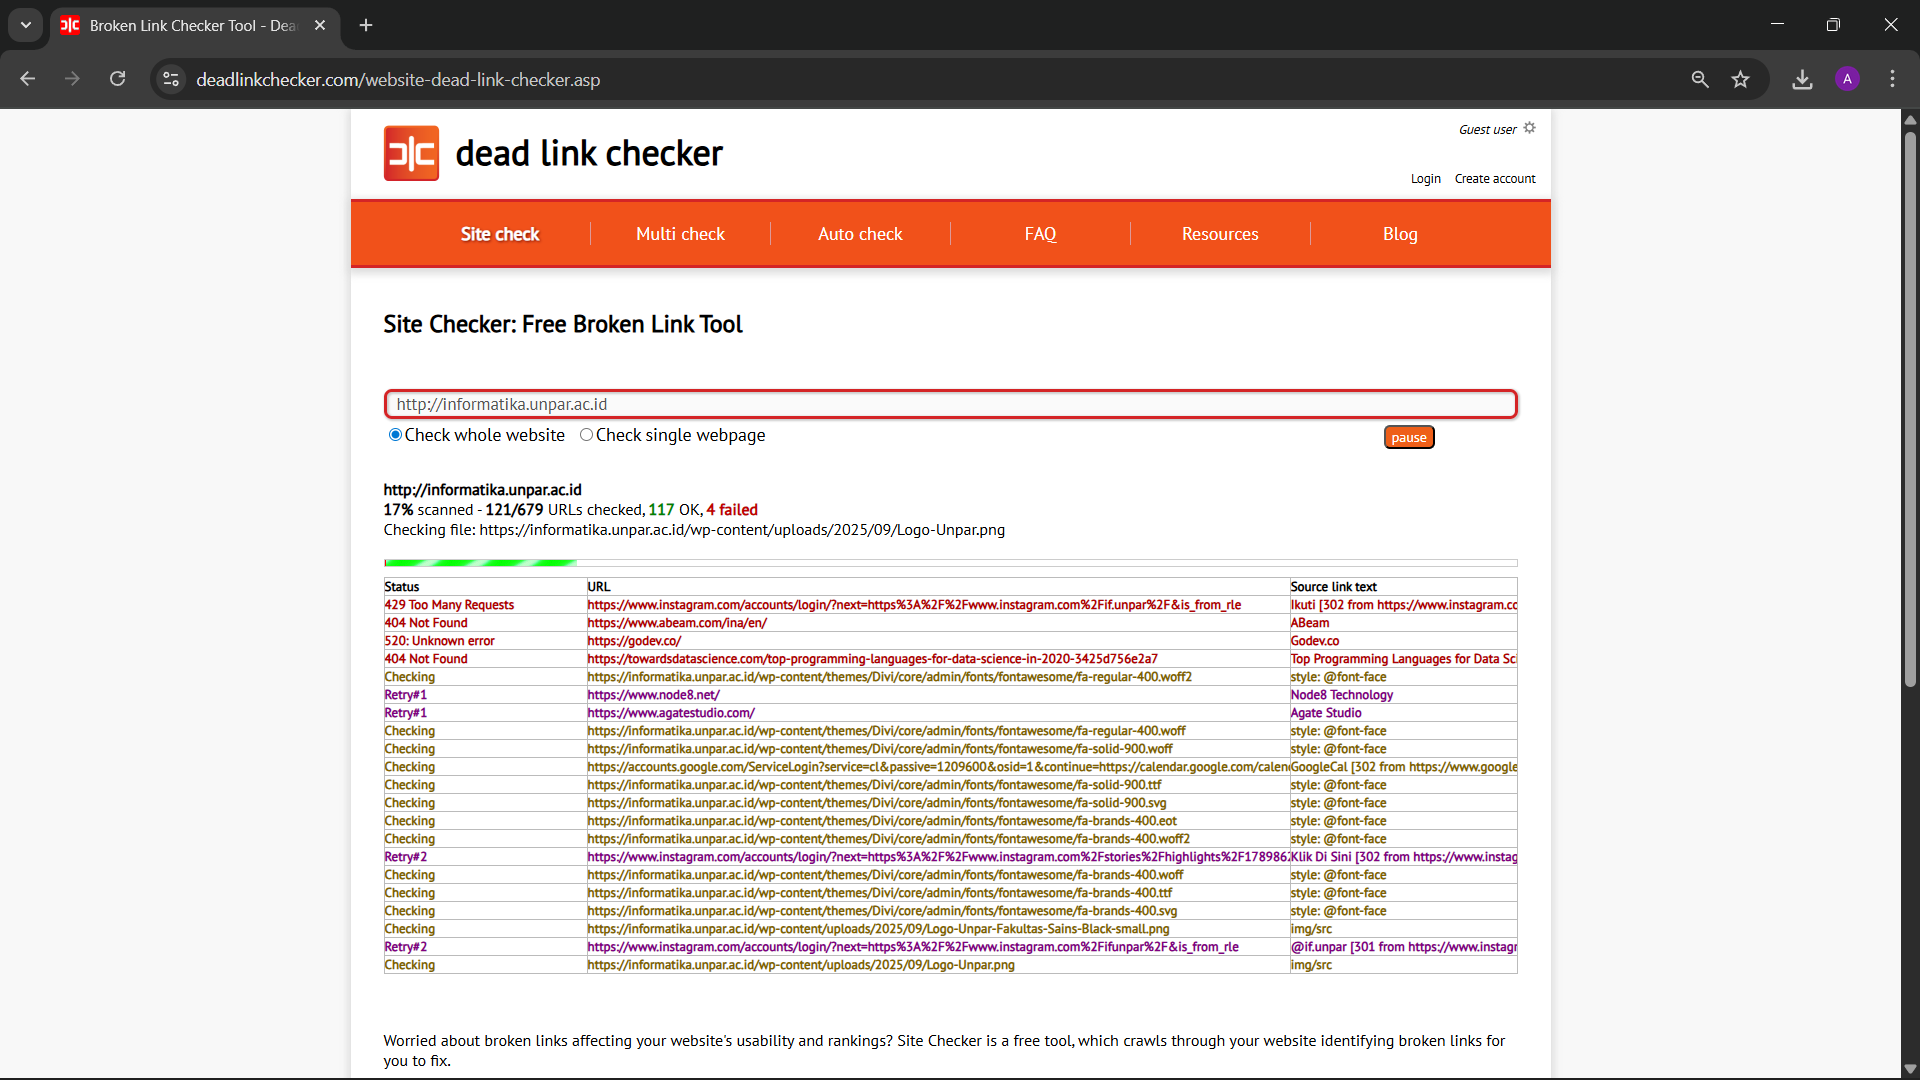
\includegraphics[width=0.9\textwidth]{Gambar/030202-dead-link-checker.png}
    \caption{Antarmuka Dead Link Checker}
    \label{fig:analisis-deadlinkchecker}
\end{figure}

Berikut adalah penjelasan komponen antarmuka pengguna pada layanan \textit{site check} :
\begin{enumerate}
    \item \textbf{Input URL}\\  
    Pengguna cukup memasukkan alamat domain atau halaman dengan URL absolut yang ingin diperiksa. Jika skema tidak dituliskan, sistem secara otomatis menambahkan awalan \texttt{http://}. Hal ini menyederhanakan input, meskipun dapat menimbulkan masalah pada situs yang hanya mendukung skema HTTPS.  

    \item \textbf{Mode pemeriksaan}\\  
    Dead Link Checker menyediakan dua opsi, yakni \textit{Check whole website} untuk menelusuri seluruh halaman dalam domain yang sama dengan URL input, dan \textit{Check single webpage} untuk memeriksa hanya halaman yang diberikan sesuai URL input.
 
    \item \textbf{Kontrol proses}\\
    Pemeriksaan tautan dijalankan dengan menekan tombol \textit{check}. Setelah proses berlangsung, tombol ini berubah menjadi \textit{pause} yang jika ditekan maka akan menghentikan sementara proses pemeriksaan dan menyimpan posisi terakhir. Pada kondisi jeda, tombol \textit{pause} akan digantikan dengan dua tombol, yaitu \textit{resume} untuk melanjutkan pemeriksaan dari titik terakhir, dan \textit{cancel} untuk membatalkan seluruh proses.

    \item \textbf{Ringkasan pemeriksaan}\\  
    Ringkasan pemeriksaan menampilkan informasi utama terkait progres yang sedang berlangsung. Bagian ini memuat alamat situs yang diperiksa, persentase pemindaian yang telah selesai, jumlah tautan yang sudah diperiksa dibandingkan dengan total tautan yang ditemukan, serta jumlah tautan yang berstatus OK dan yang \textit{failed}. Informasi tambahan juga ditampilkan berupa alamat tautan yang sedang diperiksa pada saat itu. Tepat di bawahnya terdapat \textit{progress bar} berwarna, di mana warna hijau beraksen putih menunjukkan jumlah tautan yang berstatus OK dan sedang di proses, sedangkan warna merah menunjukkan jumlah tautan yang gagal diakses.

    \item \textbf{Tabel hasil}\\
    Hasil pemeriksaan ditampilkan dalam bentuk tabel dengan tiga kolom utama yang isinya diperbarui secara langsung (\textit{real time}) selama pemeriksaan berlangsung. Tautan yang valid dihapus otomatis dari tabel setelah berhasil diperiksa, sehingga yang tersisa hanya entri yang bermasalah atau sedang diproses. Berikut adalah penjelasan untuk tiap kolom:
    \begin{itemize}
    
        \item \textbf{Status}: Pada kolom ini, awalnya semua tautan diberi status \textit{Checking}, jika pada tahap ini terjadi kegagalan koneksi atau tidak ada respons dari server, sistem secara otomatis melakukan percobaan ulang yang ditandai dengan \textit{Retry\#1} dan \textit{Retry\#2}. Apabila setelah dua kali percobaan ulang tautan tetap tidak dapat diakses, maka status akhir ditetapkan sesuai kondisi terakhir, seperti \texttt{Timeout} atau \texttt{Host not found}. Sebaliknya, jika server memberikan respons yang jelas, sistem langsung menampilkan kode hasil tanpa melakukan retry, seperti \texttt{404 Not Found}, \texttt{500 Internal Server Error}, \texttt{429 Too Many Requests}, atau kode non-standar seperti \texttt{999}. Warna latar baris juga digunakan untuk memperjelas status: kuning untuk \textit{Checking}, ungu untuk \textit{Retry}, dan merah untuk tautan yang rusak.
        
        \item \textbf{URL}: Kolom ini berisi alamat tautan yang sedang atau sudah diperiksa. Setiap entri dapat diklik untuk membuka alamat tersebut secara langsung di \textit{browser}.
        
        \item \textbf{Source link text}: Kolom ini menunjukkan teks jangkar dari tautan atau konteks halaman sumber tempat tautan ditemukan. Bagian ini juga dapat diklik untuk membuka halaman asal tautan ditemukan.
        
    \end{itemize}
\end{enumerate}

\subsubsection*{Mekanisme dan Ketentuan Teknis}  
Selain fitur yang terlihat pada antarmuka, Dead Link Checker juga memiliki mekanisme dan ketentuan teknis berikut:

\begin{enumerate}
    \item \textbf{\textit{Crawling} rekursif}\\
    Dead Link Checker bekerja dengan cara \textit{crawling} halaman web secara rekursif, yaitu dengan mengikuti setiap tautan yang ditemukan untuk kemudian dipindai kembali. Proses dimulai dari URL awal, lalu setiap tautan dalam domain yang sama diperiksa dan jika valid akan diperlakukan sebagai halaman baru untuk dianalisis. Pola ini terus diulangi hingga batas kedalaman tertentu, di mana pemeriksaan penuh (\textit{full scan}) dapat menjangkau hingga sepuluh tingkat halaman. 

    \item \textbf{Kepatuhan terhadap Robots.txt}\\
    Dead Link Checker melakukan pemindaian dengan tetap menghormati aturan pada berkas \texttt{robots.txt} yang dimiliki oleh situs web target. Pada berkas ini, administrator situs dapat menentukan direktori yang tidak boleh diakses oleh crawler atau memberi jeda antar permintaan untuk mengurangi beban server. Dead Link Checker menggunakan \textit{user-agent} khusus \texttt{www.deadlinkchecker.com}, sehingga aturan yang ditulis dengan user-agent ini akan dipatuhi. Contoh aturan yang dapat ditambahkan adalah:
    
\begin{verbatim}
User-agent: www.deadlinkchecker.com
Disallow: /shoppingbasket/
Crawl-delay: 1
\end{verbatim}

    Instruksi tersebut akan mencegah \textit{crawler} mengakses direktori \texttt{/shoppingbasket/} beserta subdirektorinya, serta memaksa jeda minimal satu detik antar permintaan. Dengan mekanisme ini, pemilik situs web memiliki kendali untuk membatasi sejauh mana Dead Link Checker dapat melakukan \textit{crawling} pada situs web mereka.

\end{enumerate}



\subsection{Broken Link Checker}
\label{subsec:0302-broken-link-checker}
Broken Link Checker\footnote{\url{https://www.brokenlinkcheck.com} (Diakses pada 30 Agustus 2025)} adalah sebuah situs web yang digunakan untuk mendeteksi tautan rusak, baik tautan internal maupun eksternal pada sebuah situs web.


\subsubsection*{Tampilan dan Interaksi}

Gambar~\ref{fig:analisis-brokenlinkchecker} menunjukkan antarmuka Broken Link Checker saat proses pemeriksaan berlangsung. Alur penggunaan secara umum dimulai dengan memasukkan alamat situs pada kolom input, mengisi kode keamanan, memilih mode pemeriksaan, lalu menekan tombol \textit{Find broken links now!} untuk memulai proses. Selama pemeriksaan berjalan, hasil ditampilkan langsung dalam bentuk tabel, dan pengguna dapat menghentikan proses dengan menekan tombol \textit{Stop}.

\begin{figure}[H]
    \centering
    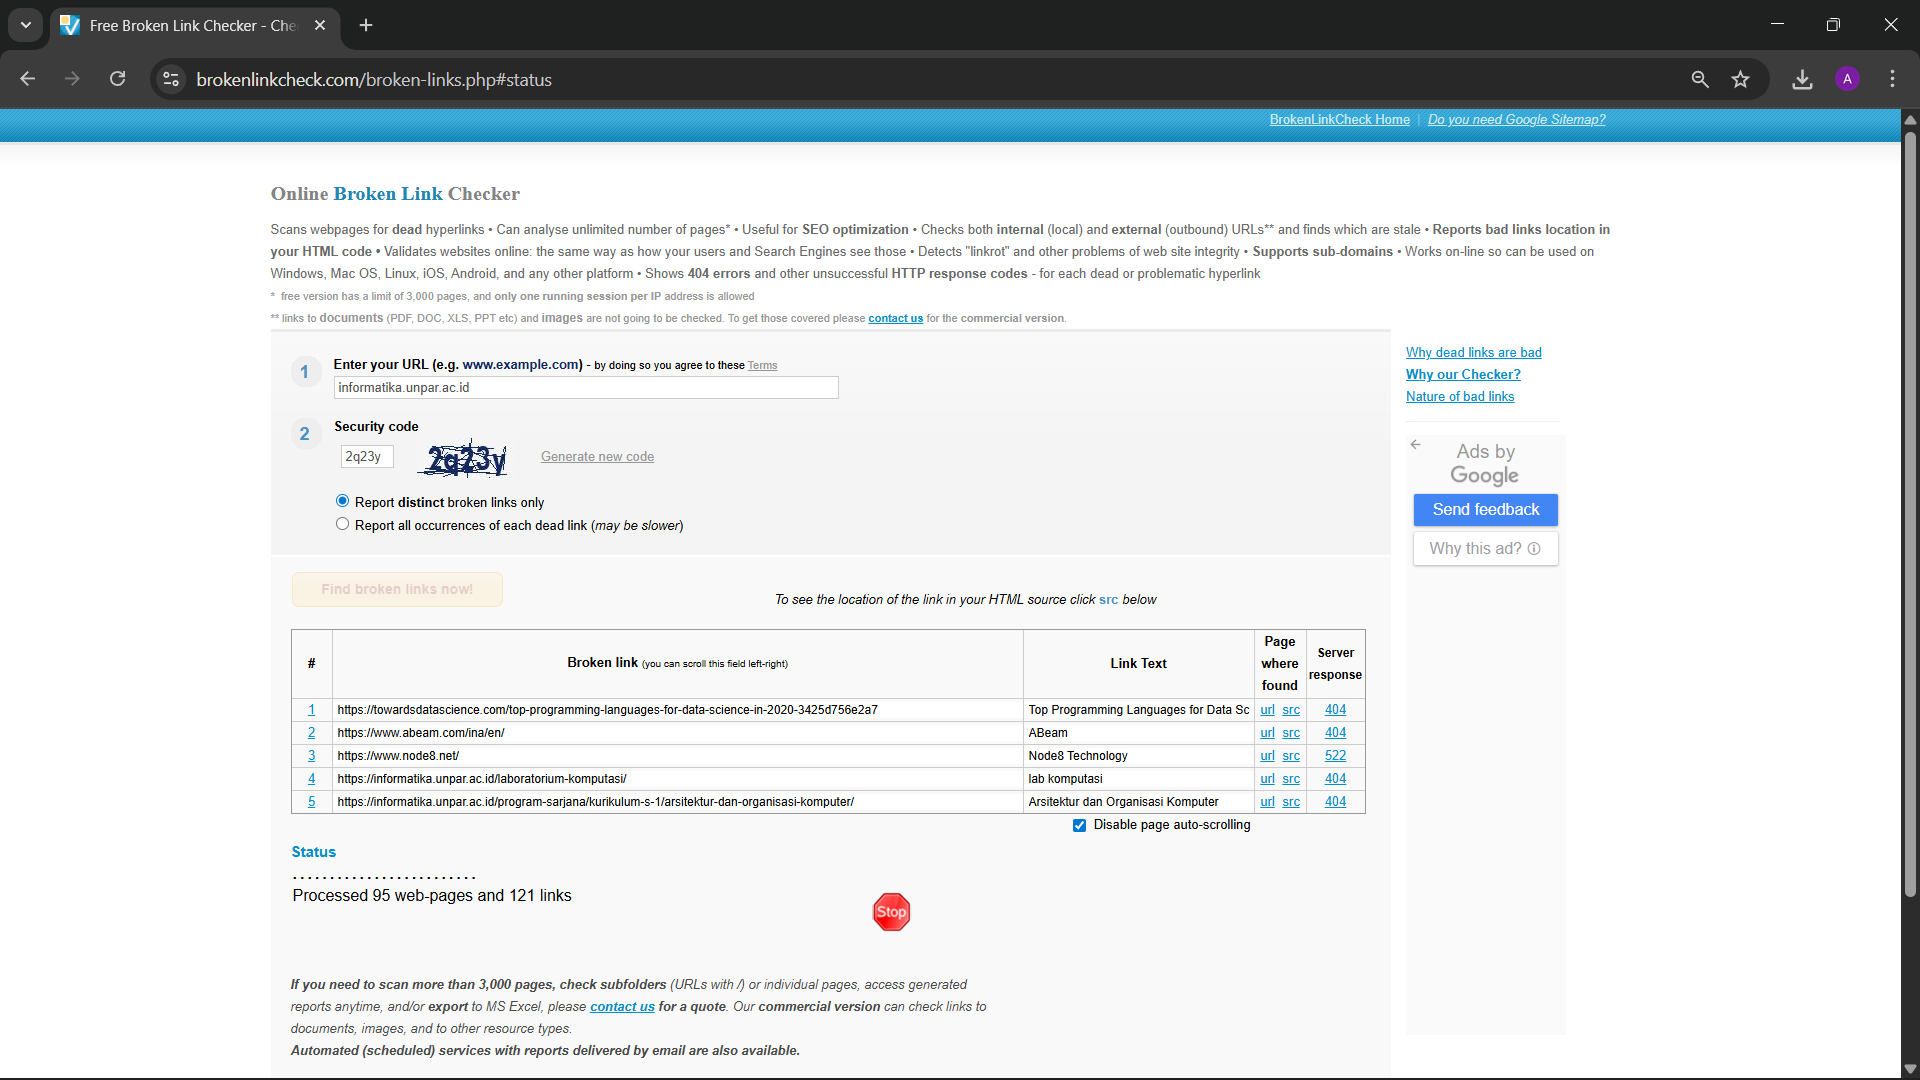
\includegraphics[width=0.95\textwidth]{Gambar/030203-broken-link-checker.png}
    \caption{Antarmuka Broken Link Checker}
    \label{fig:analisis-brokenlinkchecker}
\end{figure}

Berikut adalah komponen utama antarmuka pengguna Broken Link Checker pada layanan pemeriksaan tautan rusak:

\begin{enumerate}
    \item \textbf{Input URL}\\
    Komponen ini digunakan untuk memasukkan alamat situs web yang akan diperiksa. Pengguna dapat menuliskan alamat dalam bentuk domain saja, tanpa harus menyertakan skema \texttt{http://} atau \texttt{https://}. Sistem akan tetap menerima input tersebut dan mengolahnya sebagai URL awal pemeriksaan. Kemudahan ini mempersingkat proses input, meskipun dapat menimbulkan potensi ambiguitas pada situs web yang hanya mendukung skema tertentu, misalnya hanya \texttt{https://}.

    \item \textbf{Security code}\\
    Sebelum memulai proses pemeriksaan, pengguna diwajibkan mengisi \textit{security code} berupa captcha. Keharusan ini berfungsi sebagai mekanisme pencegahan terhadap penggunaan otomatis (bot) yang dapat membebani server layanan. Kode keamanan ini bersifat dinamis dan dapat diganti dengan menekan tombol \textit{Generate new code} yang tersedia pada antarmuka.

    \item \textbf{Mode pemeriksaan}\\
    Tersedia dua pilihan mode pemeriksaan yang dapat dipilih melalui tombol radio, yaitu \textit{Report distinct broken links only}, dan \textit{Report all occurrences of each dead link}. Mode \textit{Report distinct broken links only} menampilkan setiap tautan rusak hanya sekali, tanpa memperhatikan berapa banyak halaman yang memuat tautan tersebut. Pendekatan ini membuat proses lebih cepat, tetapi informasi lokasi kemunculan tautan hanya terbatas pada satu halaman. Sebaliknya, mode \textit{Report all occurrences of each dead link (may be slower)} menampilkan seluruh kemunculan tautan rusak beserta halaman sumbernya. Dengan demikian, jika sebuah tautan rusak terdapat pada beberapa halaman, maka akan muncul beberapa entri dengan sumber berbeda pada tabel hasil. Mode ini memberikan informasi yang lebih lengkap, namun membutuhkan waktu pemrosesan yang lebih lama.

    \item \textbf{Tombol kontrol}\\
    Proses pemeriksaan dimulai dengan menekan tombol \textit{Find broken links now!}. Setelah pemeriksaan berjalan, tombol \textit{Stop} berwarna merah akan muncul di bawah tabel hasil. Tombol ini memungkinkan pengguna menghentikan proses pemeriksaan kapan saja sesuai kebutuhan. Selain itu, disediakan pula opsi \textit{Disable page auto-scrolling} yang dapat diaktifkan untuk menonaktifkan pengguliran otomatis pada tabel hasil, sehingga tampilan tetap stabil meskipun data baru terus ditambahkan secara real-time.

    \item \textbf{Tabel hasil}\\
    Hasil pemeriksaan ditampilkan dalam bentuk tabel yang diperbarui secara langsung. Tabel ini hanya menampilkan tautan yang telah dipastikan bermasalah, sehingga laporan lebih fokus dan tidak bercampur dengan tautan valid atau sedang dalam proses pemeriksaan. Terdapat lima kolom utama pada tabel hasil, yaitu:
    
    \begin{itemize}
    
        \item \textbf{\#}: kolom nomor urut hasil. Setiap nomor dapat diklik untuk membuka tautan rusak yang bersangkutan secara langsung.
        
        \item \textbf{Broken link}: berisi alamat tautan yang teridentifikasi rusak. Tautan ini ditampilkan dalam bentuk teks biasa tanpa fungsi klik.
        
        \item \textbf{Link text}: menampilkan teks jangkar (\textit{anchor text}) dari tautan yang ditemukan, atau keterangan terkait jika tersedia.
        
        \item \textbf{Page where found}: berisi dua tautan, yaitu \textit{url} yang mengarah ke halaman web tempat tautan rusak ditemukan, serta \textit{src} yang menunjuk ke dokumen HTML sumber untuk memperlihatkan lokasi tautan yang bermasalah.
        
        \item \textbf{Server response}: menampilkan status akhir dari hasil pemeriksaan tautan, baik berupa kode status HTTP seperti \texttt{404} dan \texttt{500}, maupun pesan kesalahan non-HTTP seperti \texttt{bad host} atau \texttt{timeout}.
        
    \end{itemize}

    \item \textbf{Ringkasan pemeriksaan}\\
    Pada bagian bawah tabel, sistem menampilkan ringkasan proses pemeriksaan yang sedang berlangsung. Bagian ini memuat status terkini, yang ditandai dengan animasi titik berjalan selama proses aktif. Jika pemeriksaan dihentikan oleh pengguna melalui tombol \textit{Stop}, status akan berubah menjadi \texttt{DONE : process was terminated by user}. Sebaliknya, jika pemeriksaan selesai secara normal, status ditampilkan sebagai \texttt{COMPLETED!}. Selain menampilkan status, ringkasan ini juga memperlihatkan jumlah total halaman dan tautan yang telah diperiksa, serta jumlah tautan rusak yang ditemukan.
\end{enumerate}


\subsubsection*{Mekanisme dan Ketentuan Teknis}  
Selain fitur yang tampak pada antarmuka, Broken Link Checker juga memiliki sejumlah mekanisme teknis yang menentukan cara kerja dan batasan layanan. Mekanisme ini penting untuk dipahami agar pengguna dapat menafsirkan hasil pemeriksaan dengan tepat dan menyesuaikan penggunaan sesuai kebutuhan. Mekanisme dan ketentuan teknis tersebut dapat dirangkum sebagai berikut:

\begin{enumerate}
    \item \textbf{Cakupan pemeriksaan}\\
    Broken Link Checker melakukan pemeriksaan terhadap tautan internal maupun eksternal dari sebuah situs web. Tautan internal adalah tautan yang berada dalam domain yang sama dengan URL awal, sedangkan tautan eksternal adalah tautan yang mengarah keluar ke domain lain. Hanya tautan yang bermasalah yang ditampilkan dalam laporan, sedangkan tautan valid tidak ditampilkan. Pendekatan ini membuat hasil pemeriksaan lebih bersih dan mudah dianalisis karena pengguna tidak perlu memilah-milah tautan yang sebenarnya masih berfungsi.

    \item \textbf{Batasan versi gratis}\\
    Versi gratis dari layanan ini memiliki beberapa pembatasan. Pemeriksaan hanya dapat dilakukan hingga maksimum 3.000 halaman dalam satu sesi, dengan ketentuan satu sesi diperbolehkan untuk setiap alamat IP pada satu waktu. Selain itu, pemeriksaan pada versi gratis tidak mencakup tautan yang menuju ke dokumen seperti PDF, DOC, XLS, PPT, maupun tautan ke file gambar. Batasan ini diberlakukan untuk mengurangi beban layanan sekaligus mendorong pengguna yang membutuhkan cakupan lebih luas untuk beralih ke versi komersial.

    \item \textbf{Fitur versi komersial}\\
    Untuk kebutuhan yang lebih kompleks, Broken Link Checker menyediakan layanan berbayar dengan fitur tambahan. Pada versi ini, pemeriksaan dapat dilakukan pada jumlah halaman yang jauh lebih besar tanpa batasan ketat seperti pada versi gratis. Selain itu, layanan berbayar mendukung pemindaian sub-folder dan sub-domain, pemeriksaan tautan yang mengarah ke dokumen maupun gambar, serta ekspor hasil pemeriksaan ke format CSV atau Excel untuk memudahkan analisis lanjutan. Fitur lain yang ditawarkan mencakup pembuatan laporan otomatis yang dikirim melalui email secara terjadwal (harian, mingguan, atau bulanan), opsi konfigurasi kecepatan pemeriksaan sesuai kebutuhan situs target, serta analisis tambahan seperti pemeriksaan feed RSS atau ATOM.
\end{enumerate}
